\documentclass{THUexprep}
\usepackage{colortbl}
\usepackage{booktabs}
\usepackage{gensymb}
\usepackage{longtable}
\usepackage{multirow}
\usepackage{graphicx}
\usepackage{subcaption}
\usepackage[per-mode=symbol]{siunitx}
\sisetup{detect-all}
\usepackage{multicol}
\usepackage{float}

\begin{document}
\title{高温超导实验 - 实验报告}
\class{物理 41 班}
\name{刘乐融}
\id{2024011182}
\maketitle

\section{摘要}

本实验的原理是超导体温度特性的相关知识,意图使我们熟悉小电阻值测量、实验数据处理和不确定度评估方法. 实验通过测量液氮冷却高温超导体的温度 - 电阻特性,探究超导体的温度特性.

\section{实验原理}

1. 四引线法测量微小电阻:

四引线法是一种用于测量微小电阻的方法,其原理是通过两对引线,一对用于通电,一对用于测量电压,使得电流引线和电压引线分离,从而消除引线电阻对测量结果的影响.

2. 铂电阻的温度特性:

铂电阻的工作电流约为 \SI{1}{\milli\ampere},\SI{0}{\celsius} 时的电阻值约为 $R_{t=0\celsius}\approx\SI{100.00}{\ohm}$. 测温范围为 $\numrange{-200}{0}\celsius$ 时,铂电阻的温度特性可以用以下公式描述:

\begin{equation}
    R_t = R_0 \left[1 + A t + B t^2 + C t^3(t-100)\right]
\end{equation}

\begin{equation}
    t=\frac{-A+\sqrt{A^2-40B(0.1-0.001R_t)}}{2B}
\end{equation}

其中:

\begin{equation}
    \begin{aligned}
        A &= \SI{3.9083e-3}{\per\celsius}\\
        B &= \SI{-5.775e-7}{\per\celsius\squared}\\
        C &= \SI{-4.183e-12}{\per\celsius\cubed}
    \end{aligned}
\end{equation}

可以通过电阻值计算温度.

3. 超导体的温度特性:

超导体在转变温度以下进入超导状态. 超导状态下,超导体的电阻为零,同时出现完全抗磁性,即超导体内部的磁场为零 (Meissner Effect). Meissner Effect 使得我们能通过测量感应线圈感应电压值突变所对应的温度来确定超导体的转变温度.

\section{实验仪器及实验步骤}

本实验使用的仪器和材料有:信号发生器一台、三路稳压稳流直流电源一台、5 位半数字万用表一台、4 位半数字万用表一台、手持数字万用表一台、测试探头、测试探头接线盒、电阻板、双刀双掷开关一个、导线若干、BNC - 香蕉头导线一根、液氮.

实验步骤如下:

(1) 用四引线法测量常温下超导样品电阻:

先使用 5 位半万用表的电阻模式,测量导线的电阻数量级,之后连接导线,测量接触电阻,最后按照实验讲义上的图示连接电路,用四引线法测量超导样品在常温下的电阻.

(2) 用电流换向法消除乱真电势的影响:

用双刀双掷开关将电流换向,消除乱真电势的影响,并计算理论公式.

(3) 用铂电阻温度计测量温度:

连接电路,使用限流电阻控制电流约为铂电阻的工作电流,用 4 位半万用表和四引线法测量铂电阻的电阻值,计算温度.

(4) 用电磁感应法测超导样品对感应电压的影响:

连接主线圈和次级线圈,连接电路,用手持万用电表测量次级线圈的感应电压.

(5) 降温实验:

将超导样品放入液氮中,手机录像记录转变过程中超导样品的电压、次级线圈感应电压、铂电阻电压,测量超导样品的转变温度. 对升温过程做同样操作.

(6) 处理数据.

\section{实验数据处理}

\subsection{测量超导样品常温电阻}

连接在 5 位半万用表上的两根测试导线电阻测量值为:$\SI{0.022}{\ohm}$.

从超导探头接线盒至超导样品之间的引线电阻 $R_\text{wire}$ 的测量值为:$\SI{0.497}{\ohm}-\SI{0.022}{\ohm}=\SI{0.475}{\ohm}$.

四引线法测量室温下超导样品的电阻,调节电源 CH3 为恒流模式,输出电流为 $\SI{1}{\ampere}$,测得超导样品上的电压为 $U_\text{super}=\SI{0.164}{\milli\volt}$,因此得到超导样品的电阻为:$R_\text{super}=\SI{0.164}{\milli\ohm}$.

在此过程中,CH3 输出电压为 $\SI{527}{\milli\volt}$,这与接触电阻、导线电阻和常温超导样品电阻的总和所给出的理论值接近,为同一数量级.

\subsection{电流换向法消除乱真电势的影响}

换向得到两种电流方向的电压分别为:$U_\text{Meas1}=\SI{0.164}{\milli\volt}$,$U_\text{Meas2}=\SI{0.163}{\milli\volt}$,得到乱真电势:

\begin{equation}
    U_\text{spur} = \frac{U_\text{Meas1} - U_\text{Meas2}}{2} = \SI{0.0005}{\milli\volt}\ll U_\text{super}=\frac{U_\text{Meas1}+U_\text{Meas2}}{2}=0.1635\si{\milli\volt}
\end{equation}
\newline
乱真电势远小于电压表所示电势,可以忽略不计. 最终得到超导样品的电阻为:$R_\text{super}=\SI{0.164}{\milli\ohm}$.

\subsection{用铂电阻温度计测量温度}

估算工作电流偏差:在 $\si{77}{K}\sim$ 室温 (用 $\si{300}{K}$ 估计) 范围内,铂电阻工作电流偏差为

\begin{equation}
    \Delta I = \frac{U_{\text{CH1}}}{R+R_{t=\si{77}{K}}} - \frac{U_{\text{CH1}}}{R+R_{t=\si{300}{K}}} = \SI{8.9e-4}{\milli\ampere}
\end{equation}
\newline
这与工作电流 $\SI{1}{\milli\ampere}$ 相比偏差较小,可以忽略不计.

计算室温 (认为是 $\SI{23}{\celsius}$) 下铂电阻上的电压值:$U_{t-\text{calc}}=\SI{108.96}{\milli\volt}$.

测量实际情况下铂电阻的电压值为:$U_{t-\text{real}}=\SI{109.31}{\milli\volt}$,与计算值非常接近,可以认为室温在 $23\sim\SI{24}{\celsius}$ 之间.

\subsection{用电磁感应法测超导样品对感应电压的影响}

信号源设置:输出正弦波形,$V_{pp}=\SI{200}{\milli\volt}$,$f=\SI{700}{\hertz}$,测试常温下感应线圈电压为 $\SI{16.31}{\milli\volt}$.

\subsection{降温实验}

测量降温过程中的铂电阻电压 $U_t$,超导样品电压 $U_\text{super}$,感应电压 $U_m$,数据如下表所示:

% Table generated by Excel2LaTeX from sheet 'Sheet1'
\begin{longtable}{|c|c|c|c|c|c|}
    \caption{降温过程数据} \\
    \hline
    序号 & $U_t$ (\si{\milli\volt}) & $U_{\text{super}}$ (\si{\milli\volt})  & $U_m$ (\si{\milli\volt}) & $t$ (\si{\celsius})    & $R_\text{super}$ (\si{\milli\ohm}) \\
    \hline
    \endfirsthead
    \hline
    序号 & $U_t$ (\si{\milli\volt}) & $U_{\text{super}}$ (\si{\milli\volt})  & $U_m$ (\si{\milli\volt}) & $t$ (\si{\celsius})    & $R_\text{super}$ (\si{\milli\ohm}) \\
    \hline
    \endhead
    1     & 41    & 0.076 & 18.63 & -1.48E+02 & 0.076 \\
    \hline
    2     & 40.1  & 0.075 & 18.69 & -1.50E+02 & 0.075 \\
    \hline
    3     & 39.2  & 0.074 & 18.76 & -1.52E+02 & 0.074 \\
    \hline
    4     & 38.4  & 0.073 & 18.77 & -1.54E+02 & 0.073 \\
    \hline
    5     & 37.6  & 0.073 & 18.81 & -1.56E+02 & 0.073 \\
    \hline
    6     & 36.8  & 0.072 & 18.83 & -1.58E+02 & 0.072 \\
    \hline
    7     & 36    & 0.071 & 18.88 & -1.60E+02 & 0.071 \\
    \hline
    8     & 35.9  & 0.07  & 18.91 & -1.60E+02 & 0.07 \\
    \hline
    9     & 35.8  & 0.068 & 18.92 & -1.60E+02 & 0.068 \\
    \hline
    10    & 35.7  & 0.064 & 18.9  & -1.61E+02 & 0.064 \\
    \hline
    11    & 35.6  & 0.06  & 18.93 & -1.61E+02 & 0.06 \\
    \hline
    12    & 35.5  & 0.05  & 18.89 & -1.61E+02 & 0.05 \\
    \hline
    13    & 35.4  & 0.041 & 18.92 & -1.61E+02 & 0.041 \\
    \hline
    14    & 35.3  & 0.037 & 18.94 & -1.62E+02 & 0.037 \\
    \hline
    15    & 35.2  & 0.027 & 18.9  & -1.62E+02 & 0.027 \\
    \hline
    16    & 35.1  & 0.023 & 18.91 & -1.62E+02 & 0.023 \\
    \hline
    17    & 35    & 0.021 & 18.94 & -1.62E+02 & 0.021 \\
    \hline
    18    & 34.9  & 0.02  & 18.93 & -1.63E+02 & 0.02 \\
    \hline
    19    & 34.8  & 0.02  & 18.95 & -1.63E+02 & 0.02 \\
    \hline
    20    & 33.9  & 0.019 & 18.95 & -1.65E+02 & 0.019 \\
    \hline
    21    & 33.1  & 0.019 & 19.03 & -1.67E+02 & 0.019 \\
    \hline
    22    & 32.3  & 0.019 & 19.03 & -1.69E+02 & 0.019 \\
    \hline
    23    & 31.5  & 0.018 & 19.1  & -1.71E+02 & 0.018 \\
    \hline
    24    & 30.6  & 0.018 & 19.09 & -1.73E+02 & 0.018 \\
    \hline
    25    & 29.8  & 0.018 & 19.12 & -1.75E+02 & 0.018 \\
    \hline
    26    & 29    & 0.019 & 19.11 & -1.77E+02 & 0.019 \\
    \hline
    27    & 28    & 0.019 & 19.12 & -1.79E+02 & 0.019 \\
    \hline
    28    & 27.4  & 0.02  & 19.12 & -1.81E+02 & 0.02 \\
    \hline
    29    & 26.4  & 0.02  & 19.11 & -1.83E+02 & 0.02 \\
    \hline
    30    & 26.2  & 0.02  & 19.08 & -1.84E+02 & 0.02 \\
    \hline
    31    & 26.1  & 0.02  & 19.03 & -1.84E+02 & 0.02 \\
    \hline
    32    & 26    & 0.02  & 18.98 & -1.84E+02 & 0.02 \\
    \hline
    33    & 25.9  & 0.02  & 18.94 & -1.85E+02 & 0.02 \\
    \hline
    34    & 25.8  & 0.02  & 18.88 & -1.85E+02 & 0.02 \\
    \hline
    35    & 25.7  & 0.02  & 18.66 & -1.85E+02 & 0.02 \\
    \hline
    36    & 25.6  & 0.02  & 18.5  & -1.85E+02 & 0.02 \\
    \hline
    37    & 25.5  & 0.02  & 18.38 & -1.86E+02 & 0.02 \\
    \hline
    38    & 25.4  & 0.019 & 18.05 & -1.86E+02 & 0.019 \\
    \hline
    39    & 25.3  & 0.019 & 17.89 & -1.86E+02 & 0.019 \\
    \hline
    40    & 25.2  & 0.02  & 17.57 & -1.86E+02 & 0.02 \\
    \hline
    41    & 25.1  & 0.02  & 17.37 & -1.87E+02 & 0.02 \\
    \hline
    42    & 25    & 0.02  & 17.07 & -1.87E+02 & 0.02 \\
    \hline
    43    & 24.9  & 0.02  & 16.83 & -1.87E+02 & 0.02 \\
    \hline
    44    & 24.8  & 0.02  & 16.56 & -1.87E+02 & 0.02 \\
    \hline
    45    & 24.7  & 0.02  & 16.35 & -1.87E+02 & 0.02 \\
    \hline
    46    & 24.6  & 0.02  & 16.07 & -1.88E+02 & 0.02 \\
    \hline
    47    & 24.5  & 0.019 & 15.89 & -1.88E+02 & 0.019 \\
    \hline
    48    & 24.4  & 0.019 & 15.52 & -1.88E+02 & 0.019 \\
    \hline
    49    & 24.3  & 0.019 & 15.43 & -1.88E+02 & 0.019 \\
    \hline
    50    & 24.2  & 0.019 & 15.09 & -1.89E+02 & 0.019 \\
    \hline
    51    & 24.1  & 0.019 & 14.98 & -1.89E+02 & 0.019 \\
    \hline
    52    & 24    & 0.019 & 14.7  & -1.89E+02 & 0.019 \\
    \hline
    53    & 23.9  & 0.019 & 14.45 & -1.89E+02 & 0.019 \\
    \hline
    54    & 23.8  & 0.02  & 14.31 & -1.90E+02 & 0.02 \\
    \hline
    55    & 23.7  & 0.02  & 14.08 & -1.90E+02 & 0.02 \\
    \hline
    56    & 23.6  & 0.02  & 13.99 & -1.90E+02 & 0.02 \\
    \hline
\end{longtable}

计算铂电阻电压所对应的温度和超导样品电阻,填入上表中,最终可以作出超导电阻 - 温度 ($R_\text{super}$ - $t$) 关系图和感应电压 - 温度 ($U_m$ - $t$) 关系图,如下:

\begin{figure}[H]
    \centering
    \begin{subfigure}{0.45\textwidth}
        \centering
        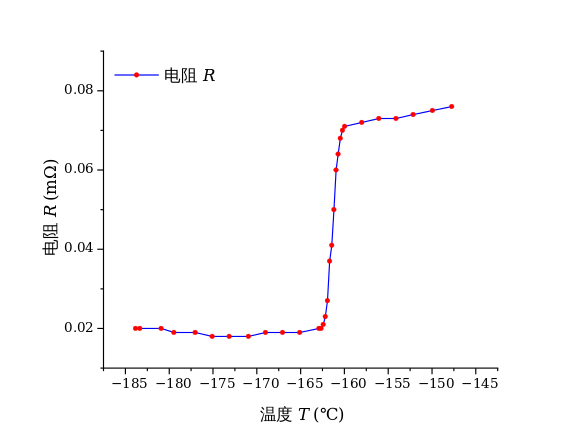
\includegraphics[width=\textwidth]{R-T1.png}
        \caption{$R_\text{super}$ - $t$ 关系}
    \end{subfigure}
    \begin{subfigure}{0.45\textwidth}
        \centering
        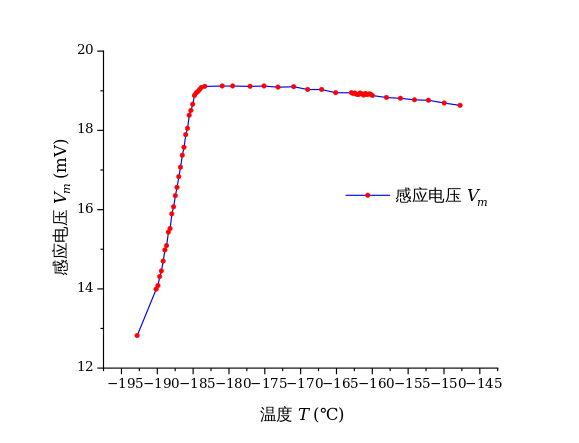
\includegraphics[width=\textwidth]{V_m-T1.png}
        \caption{$U_m$ - $t$ 关系}
    \end{subfigure}
    \caption{降温过程数据图}
\end{figure}

其中,$R$ - $T$ 关系图只用到了前 $30$ 组数据,因为在 $30$ 组数据之后,超导电阻上的电压并没有特别大的变化. 同时,图上的连线使用的是 Origin Pro 软件中的样条连接图.

由图,得到两种转变温度 $T_c$ 的测量结果:$T_{cR}=\SI{-163}{\celsius}$,$T_{cV}=\SI{-187}{\celsius}$.

转变温度宽度:$\Delta T_{cR} = \SI{2.5}{\celsius}$,$\Delta T_{cV}=\SI{4.5}{\celsius}$.

升温数据如下:

% Table generated by Excel2LaTeX from sheet 'Sheet1'
\begin{longtable}{|c|c|c|c|c|c|}
    \caption{升温过程数据} \\
    \hline
    序号 & $U_t$ (\si{\milli\volt}) & $U_{\text{super}}$ (\si{\milli\volt})  & $U_m$ (\si{\milli\volt}) & $t$ (\si{\celsius})    & $R_\text{super}$ (\si{\milli\ohm}) \\
    \hline
    \endfirsthead
    \hline
    序号 & $U_t$ (\si{\milli\volt}) & $U_{\text{super}}$ (\si{\milli\volt})  & $U_m$ (\si{\milli\volt}) & $t$ (\si{\celsius})    & $R_\text{super}$ (\si{\milli\ohm}) \\
    \hline
    \endhead
    \hline
    1     & 23.6  & 0.021 & 12.55 & -1.90E+02 & -0.001 \\
    \hline
    2     & 24.5  & 0.021 & 12.58 & -1.88E+02 & -0.001 \\
    \hline
    3     & 25.3  & 0.021 & 12.62 & -1.86E+02 & -0.001 \\
    \hline
    4     & 26.1  & 0.021 & 12.69 & -1.84E+02 & -0.001 \\
    \hline
    5     & 27    & 0.02  & 12.86 & -1.82E+02 & 0 \\
    \hline
    6     & 27.8  & 0.02  & 13.09 & -1.80E+02 & 0 \\
    \hline
    7     & 28.6  & 0.02  & 13.52 & -1.78E+02 & 0 \\
    \hline
    8     & 28.7  & 0.019 & 13.58 & -1.78E+02 & 0.001 \\
    \hline
    9     & 28.8  & 0.02  & 13.66 & -1.78E+02 & 0 \\
    \hline
    10    & 28.9  & 0.019 & 13.77 & -1.77E+02 & 0.001 \\
    \hline
    11    & 29    & 0.019 & 13.86 & -1.77E+02 & 0.001 \\
    \hline
    12    & 29.1  & 0.019 & 13.93 & -1.77E+02 & 0.001 \\
    \hline
    13    & 29.2  & 0.019 & 14.03 & -1.77E+02 & 0.001 \\
    \hline
    14    & 29.5  & 0.019 & 14.17 & -1.76E+02 & 0.001 \\
    \hline
    15    & 29.6  & 0.019 & 14.39 & -1.76E+02 & 0.001 \\
    \hline
    16    & 29.7  & 0.019 & 14.51 & -1.75E+02 & 0.001 \\
    \hline
    17    & 29.8  & 0.018 & 14.63 & -1.75E+02 & 0.002 \\
    \hline
    18    & 29.9  & 0.018 & 14.74 & -1.75E+02 & 0.002 \\
    \hline
    19    & 30    & 0.019 & 14.94 & -1.75E+02 & 0.001 \\
    \hline
    20    & 30.1  & 0.019 & 15.04 & -1.74E+02 & 0.001 \\
    \hline
    21    & 30.2  & 0.018 & 15.36 & -1.74E+02 & 0.002 \\
    \hline
    22    & 30.3  & 0.018 & 15.51 & -1.74E+02 & 0.002 \\
    \hline
    23    & 30.4  & 0.018 & 15.69 & -1.74E+02 & 0.002 \\
    \hline
    24    & 30.5  & 0.018 & 15.94 & -1.73E+02 & 0.002 \\
    \hline
    25    & 30.6  & 0.018 & 16.22 & -1.73E+02 & 0.002 \\
    \hline
    26    & 30.7  & 0.018 & 16.4  & -1.73E+02 & 0.002 \\
    \hline
    27    & 30.8  & 0.018 & 16.59 & -1.73E+02 & 0.002 \\
    \hline
    28    & 30.9  & 0.017 & 16.76 & -1.72E+02 & 0.003 \\
    \hline
    29    & 31    & 0.017 & 17.04 & -1.72E+02 & 0.003 \\
    \hline
    30    & 31.1  & 0.017 & 17.34 & -1.72E+02 & 0.003 \\
    \hline
    31    & 31.2  & 0.017 & 17.72 & -1.72E+02 & 0.003 \\
    \hline
    32    & 31.3  & 0.017 & 17.95 & -1.71E+02 & 0.003 \\
    \hline
    33    & 31.4  & 0.016 & 18.22 & -1.71E+02 & 0.004 \\
    \hline
    34    & 31.5  & 0.016 & 18.72 & -1.71E+02 & 0.004 \\
    \hline
    35    & 31.6  & 0.015 & 18.95 & -1.71E+02 & 0.005 \\
    \hline
    36    & 31.7  & 0.008 & 19.04 & -1.70E+02 & 0.012 \\
    \hline
    37    & 31.9  & 0.004 & 19.11 & -1.70E+02 & 0.016 \\
    \hline
    38    & 32    & -0.003 & 19.13 & -1.70E+02 & 0.023 \\
    \hline
    39    & 32.1  & -0.018 & 19.19 & -1.69E+02 & 0.038 \\
    \hline
    40    & 32.2  & -0.022 & 19.21 & -1.69E+02 & 0.042 \\
    \hline
    41    & 32.3  & -0.026 & 19.19 & -1.69E+02 & 0.046 \\
    \hline
    42    & 32.4  & -0.03 & 19.17 & -1.69E+02 & 0.05 \\
    \hline
    43    & 32.5  & -0.034 & 19.12 & -1.69E+02 & 0.054 \\
    \hline
    44    & 32.6  & -0.037 & 19.15 & -1.68E+02 & 0.057 \\
    \hline
    45    & 33.6  & -0.038 & 19.1  & -1.66E+02 & 0.058 \\
    \hline
    46    & 34.4  & -0.04 & 19.04 & -1.64E+02 & 0.06 \\
    \hline
    47    & 35.2  & -0.041 & 19.06 & -1.62E+02 & 0.061 \\
    \hline
    48    & 36    & -0.043 & 19.01 & -1.60E+02 & 0.063 \\
    \hline
    49    & 36.8  & -0.044 & 18.99 & -1.58E+02 & 0.064 \\
    \hline
    50    & 37.6  & -0.045 & 18.97 & -1.56E+02 & 0.065 \\
    \hline
    51    & 38.4  & -0.046 & 18.92 & -1.54E+02 & 0.066 \\
    \hline
    52    & 39.2  & -0.048 & 18.91 & -1.52E+02 & 0.068 \\
    \hline
    53    & 40.1  & -0.05 & 18.87 & -1.50E+02 & 0.07 \\
    \hline
    54    & 40.8  & -0.051 & 18.83 & -1.48E+02 & 0.071 \\
    \hline
    55    & 41.7  & -0.052 & 18.77 & -1.46E+02 & 0.072 \\
    \hline
    56    & 42.5  & -0.054 & 18.73 & -1.44E+02 & 0.074 \\
    \hline
    57    & 43.3  & -0.055 & 18.71 & -1.42E+02 & 0.075 \\
    \hline
\end{longtable}

其中 $R_\text{super}$ 已经扣除了乱真电势的影响,并且这一次的样品电压测量数据反向了 (因为在超导状态时为了测试是否真正达到超导反接了电压表). 同样画出图像:

\begin{figure}[H]
    \centering
    \begin{subfigure}{0.45\textwidth}
        \centering
        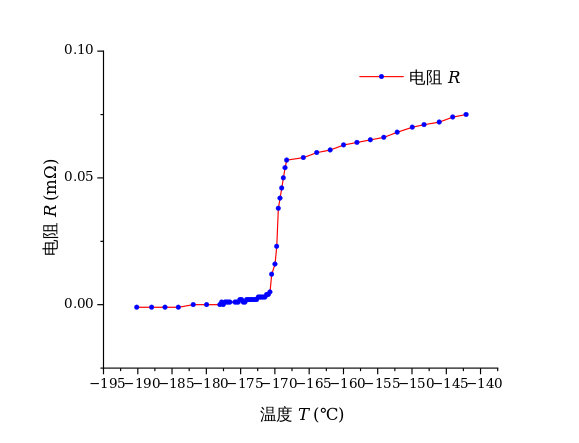
\includegraphics[width=\textwidth]{R-T2.png}
        \caption{$R_\text{super}$ - $t$ 关系}
    \end{subfigure}
    \begin{subfigure}{0.45\textwidth}
        \centering
        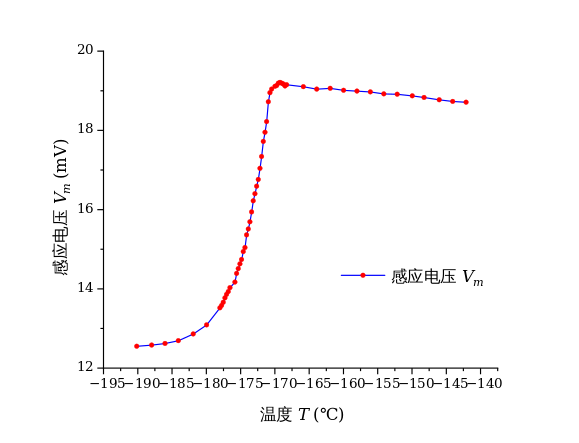
\includegraphics[width=\textwidth]{V_m-T2.png}
        \caption{$U_m$ - $t$ 关系}
    \end{subfigure}
    \caption{升温过程数据图}
\end{figure}

得到两种转变温度测量数据:$T'_{cR}=\SI{-167}{\celsius}$,$T'_{cV}=\SI{-175}{\celsius}$.

转变温度宽度:$\Delta T'_{cR} = \SI{2.5}{\celsius}$,$\Delta T'_{cV}=\SI{7.5}{\celsius}$.

因为升温过程中铂电阻和超导样品的导热较好,所以采用升温过程中的数据,得到最终结果为:$T_c=\SI{-171}{\celsius}$,$\Delta T_c=\SI{5.5}{\celsius}$.

\section{分析与讨论}

在实验过程中明显发现一个问题:感应电压和超导电阻的转变温度不一致.

我认为,原因如下:实验中使用的超导样品不是完美的,其中的缺陷导致即使某一处已经电阻为零 (这导致总电阻为零,因为相当于并联),超导体本身也不是完全抗磁性的,磁力线仍然能穿过部分超导体,所以整个超导体变为完全抗磁的情况需要的温度更低、时间更长.

同时实验中不只有这一种误差,误差还有可能来自于铂电阻和超导样品之间的导热性不够良好,导致铂电阻的温度和超导样品的温度不一致.

\section{原始数据截图}

\begin{figure}[H]
    \centering
    \begin{subfigure}{0.45\textwidth}
        \centering
        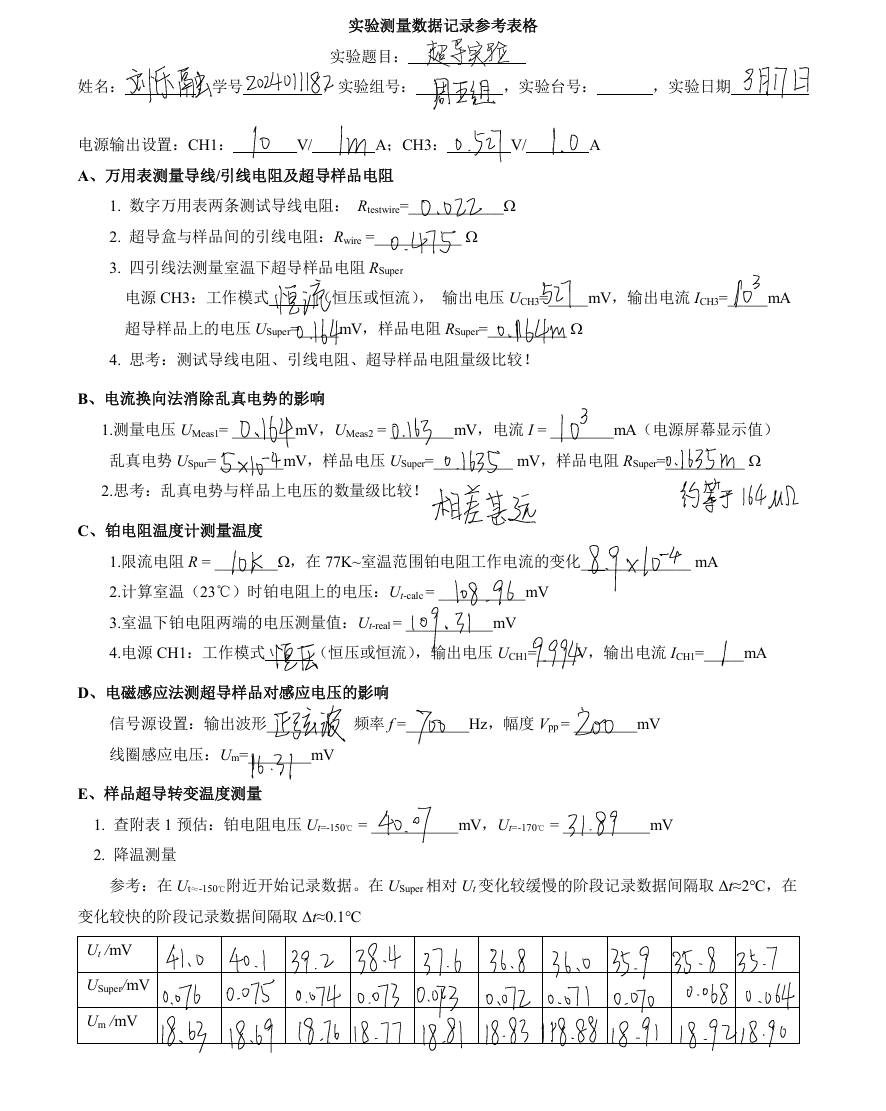
\includegraphics[width=\textwidth]{1.png}
        \caption{图片 1}
    \end{subfigure}
    \begin{subfigure}{0.45\textwidth}
        \centering
        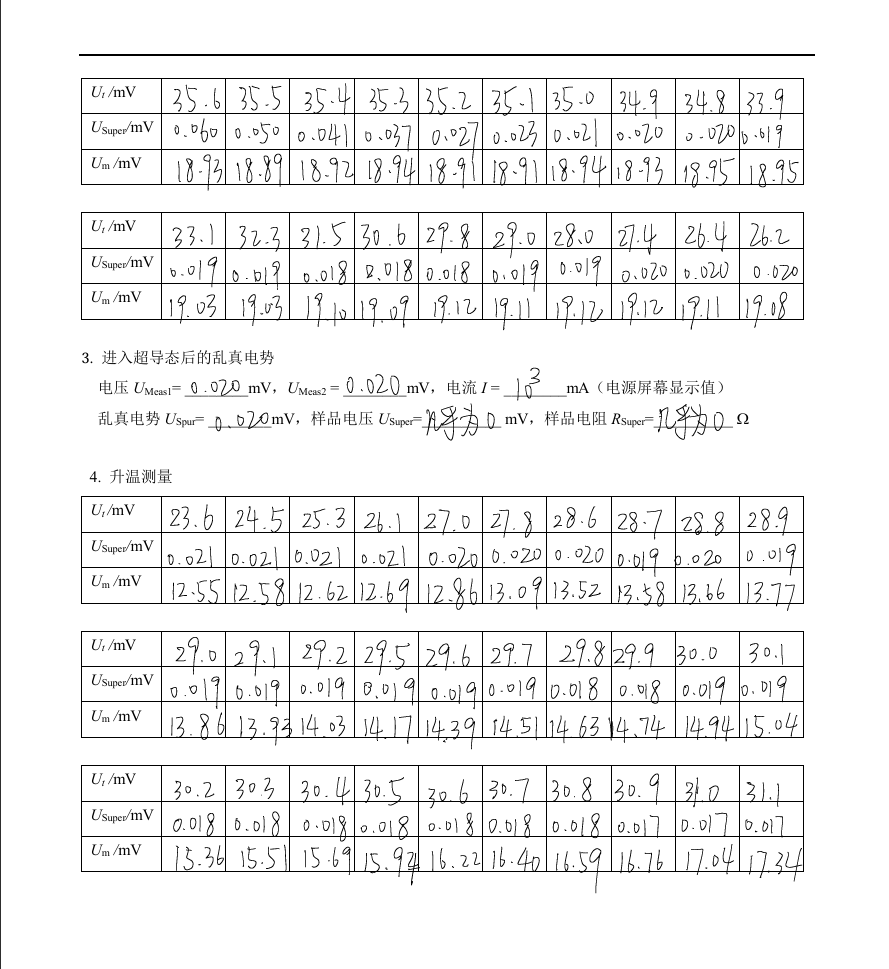
\includegraphics[width=\textwidth]{2.png}
        \caption{图片 2}
    \end{subfigure}
    \caption{实验原始数据截图 1}
\end{figure}
\begin{figure}[H]
    \begin{subfigure}{0.45\textwidth}
        \centering
        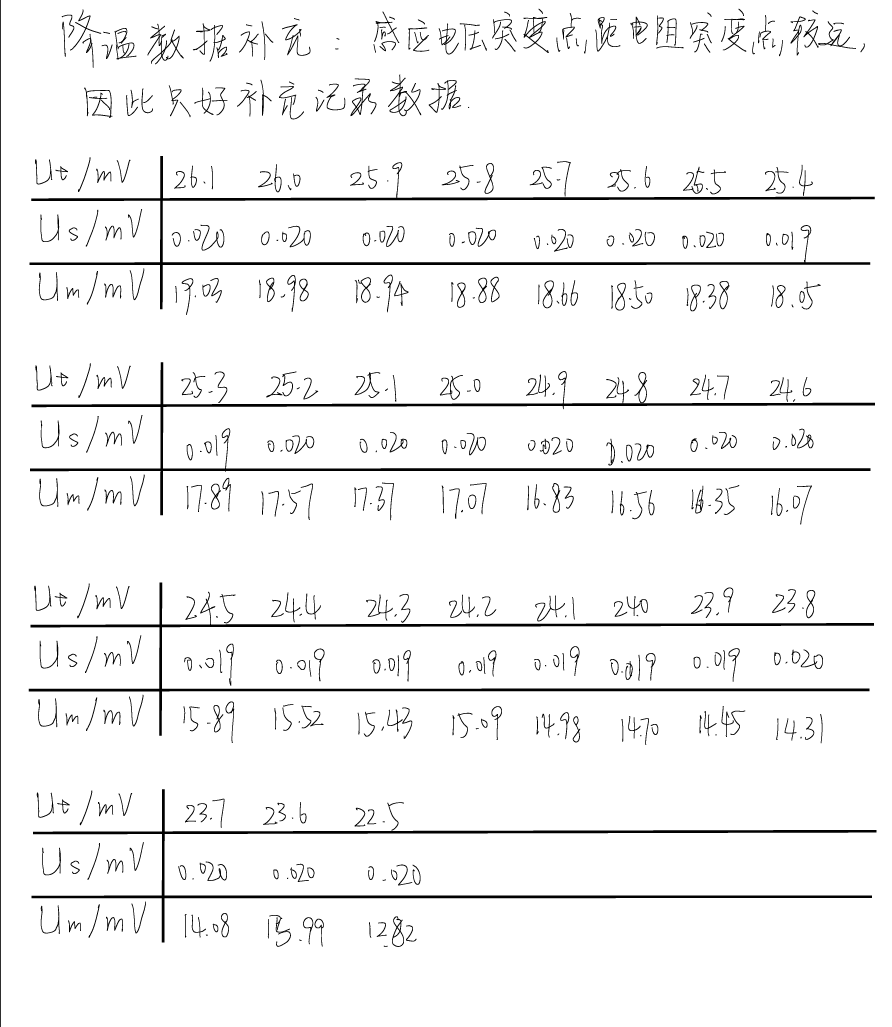
\includegraphics[width=\textwidth]{3.png}
        \caption{图片 3}
    \end{subfigure}
    \begin{subfigure}{0.45\textwidth}
        \centering
        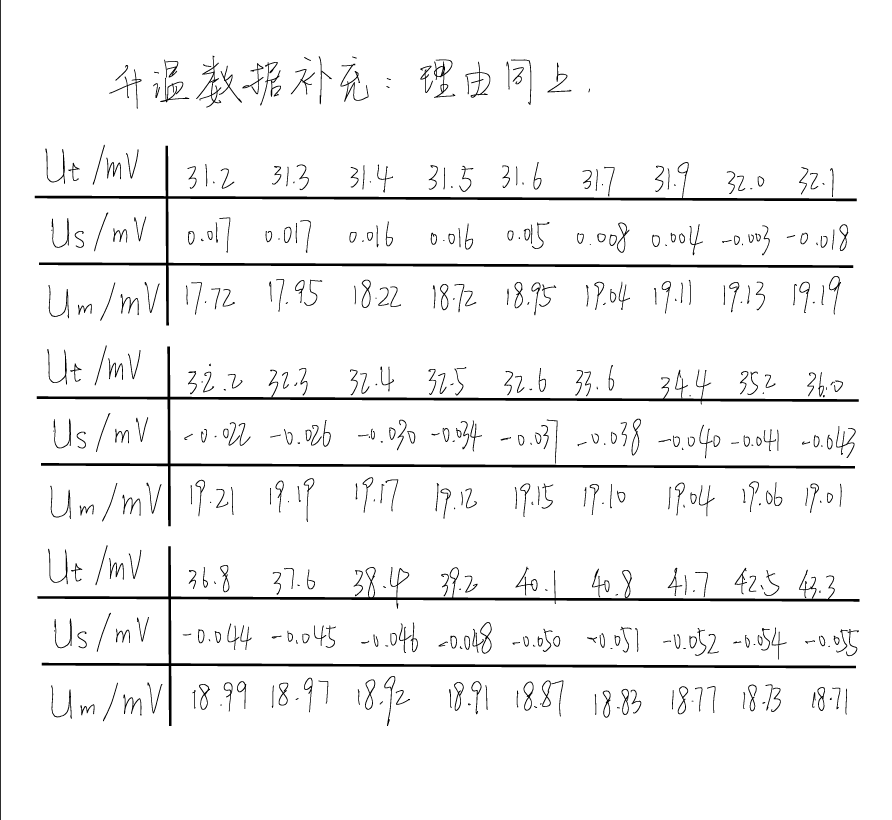
\includegraphics[width=\textwidth]{4.png}
        \caption{图片 4}
    \end{subfigure}
    \caption{实验原始数据截图 2}
\end{figure}

\end{document}